\section{Predicting Motion}
\label{sec:PredictingMotion}

To track objects in a video, there is a requirement to resolve the object's position in two consecutive frames. An ineffective brute-force approach would be to exploit the matching technique in the pixel space of the entire image, imposing an extreme computational overhead~\cite{Jalal2012}. Generally speaking, it is safe to assume that the object does not change its position abruptly. In case of vehicles, this is even more so. Tracking a jumping ball in a room that is constantly bouncing off the walls presents a greater challenge in terms of sudden change in trajectory than tracking a vehicle. Given this assumption, a physical model of the object can be utilized to reduce the region in the frame where the object should be searched for. Moreover, having a physical model backing up the visual tracking is essential as it may help determine potential failure if predictions of physical as well as visual models do not match up to a specific degree of confidence.

As we have mentioned numerous times, occlusion handling is of primary concern for us, and being able to predict a probability distribution over possible object's positions if visual input is absent is vital. We could potentially use filtering approaches, specifically Kalman filter (section~\ref{ssec:KalmanFiler}) or particle filter (section~\ref{ssec:ParticleFilter}) described later. These algorithms could model the vehicle's speed and acceleration. Filtering is an engineering terminology describing the extraction of information about a signal from partial and noisy observations (measurements)~\cite{Kunsch2013}.

% ##################################################
\subsection{Trivial Motion Model}
\label{ssec:TrivialMotionModel}

For the sake of completeness, here we describe the most trivial form of a motion predictor. This model exploits the most recent observation and linearly extrapolates the future position~\cite{broida1986estimation}.

Let $\func{p}{t}$ be the current position at time $t$, and $\func{v}{t}$ be the current velocity at time $t$ approximated as $\func{v}{t} = \func{p}{t} - \func{p}{t - 1}$. The predicted future position $\func{p}{t + 1}$ is therefore defined as

\begin{equation}
    \label{eq:TrivialMotionModel}
    \func{p}{t + 1} = \func{p}{t} + \func{v}{t} = 2\func{p}{t} - \func{p}{t - 1}.
\end{equation}

% ##################################################
\subsection{Kalman Filter}
\label{ssec:KalmanFiler}

Kalman filter~\cite{Kalman1960, welch1995introduction} is a linear predictive filter and widely applied in the computer vision community for object tracking~\cite{Jalal2012}. It has proven to be good at predicting the state in the presence of noise. This noise has to be of Gaussian probability distribution for the best performance, which can be viewed as a disadvantage in many practical, nonlinear scenarios. However, to handle such situations, the Extended Kalman Filter was proposed~\cite{welch1995introduction}, a nonlinear version of the original Kalman Filter. The major contribution is that the state transition and observation models do not need to be linear functions of the state, but they may be nonlinear instead.

Kalman Filter consists of two steps, namely \emph{prediction}, and \emph{correction} (see Fig.~\ref{fig:KalmanFilterDiagram}). In the prediction phase, the future system's state is predicted using only the variables describing the previous state. Later on, when a new observation is made, the correction step ensues and the internal state variables are updated accordingly.

Another problematic property of the Kalman Filter is its inability to simultaneously model multiple hypotheses~\cite{welch1995introduction}. This is due to the inherent, unimodal nature of the Gaussian probability distribution. This limitation is overcome by the particle Filter (section~\ref{ssec:ParticleFilter}) discussed next.

State estimation of linear dynamical systems can be performed using the Kalman Filter~\cite{kim2018introduction}. Let $t$ denote the time. The evolution of the state from time $t - 1$ to time $t$ in the process model is given by
\begin{equation}
    \vect{x}_t = \mtx{F} \vect{x}_{t - 1} + \mtx{B} \vect{u}_{t - 1} + \vect{w}_{t - 1},
\end{equation}
where $\mtx{F}$ is the state transition matrix, $\vect{x}_{t - 1}$ is the previous state vector, $\mtx{B}$ is the control-input matrix, $\vect{u}_{t - 1}$ is the control vector, and $\vect{w}_{t - 1}$, such that $\vect{w}_{t - 1} \sim \mathcal{N} \rbrackets{0, \mtx{Q}}$, is the noise vector. The assumption is that the noise is of Gaussian probability distribution with zero mean and a corresponding covariance matrix $\mtx{Q}$~\cite{kim2018introduction}.

Since the internal process model is periodically updated as new observations (measurements) are obtained, let us define the measurement vector $\vect{z}_t$ at time $t$ as
\begin{equation}
    \vect{z}_t = \mtx{H} \vect{x}_t + \vect{v}_t,
\end{equation}
with $\mtx{H}$ being the measurement matrix, $\vect{v}_t$, such that $\vect{v}_{t} \sim \mathcal{N} \rbrackets{0, \mtx{R}}$, be a zero mean, normally distributed noise vector with a related covariance matrix $\mtx{R}$~\cite{kim2018introduction}.

In this regard, the role of the Kalman Filter is to compute an estimate of the state vector $\vect{x}_t$, provided some initial estimate $\vect{x}_0$, followed by series of individual measurements, $\vect{z}_1, \vect{z}_2, \dots, \vect{z}_t$ (see Fig.~\ref{fig:KalmanFilterDiagram}). The system's behavior and state are described by matrices $\mtx{F}, \mtx{B}, \mtx{H}, \mtx{Q}$ and $\mtx{R}$, which are assumed to be time-invariant (hence the absence of indexing). Furthermore, the real covariance captured by matrices $\mtx{Q}$ and $\mtx{R}$ is also unknown, which means that the user can consider these matrices as adjustable parameters to reach the desired performance~\cite{kim2018introduction}.

\begin{figure}[t]
    \centerline{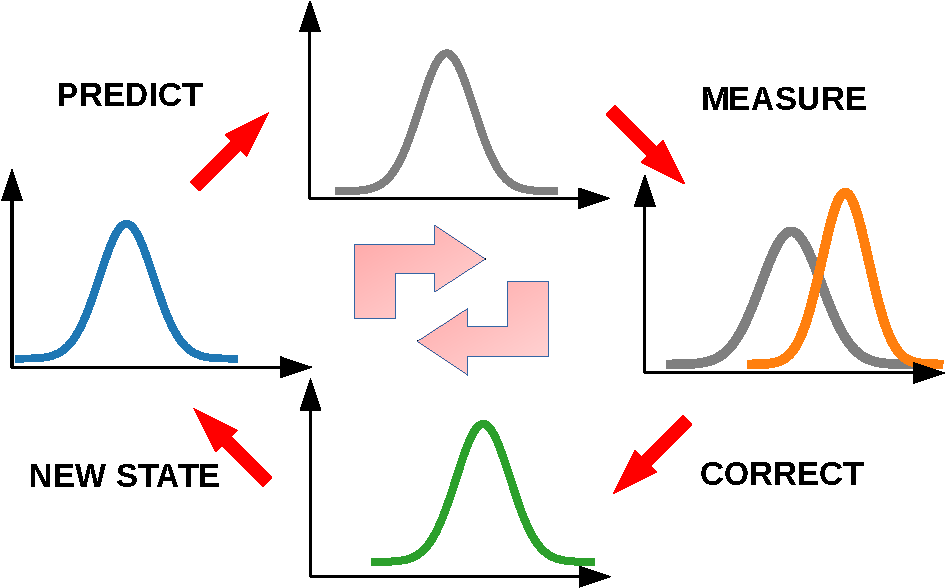
\includegraphics[width=0.7\linewidth]{figures/theoretical_foundations/kalman_filter_diagram.pdf}}
    \caption[A single iteration of the Kalman Filter]{Visualization of a single step of the Kalman Filter algorithm. Given some current state, the step begins with a prediction of the next state, then executing a measurement (in different literature a.k.a. making an observation), correcting the previous prediction in light of the newly gathered information, and in the end, using the updated variables as a basis for the next state in the future.}
    \label{fig:KalmanFilterDiagram}
\end{figure}

It is important to note that when dealing with object tracking, the Kalman Filter performs poorly in the presence of significant background clutter (spurious measurements not relating to any particular target). Clutter may introduce multimodal probability distributions over noise, which is tricky to cope with, given the already mentioned unimodal, Gaussian nature of the Kalman Filter. This realization led to the development of the Condensation (Conditional Density Propagation) algorithm, which detects and tracks objects contours in a cluttered environment~\cite{isard1998condensation}. However, this approach is outside of our scope, it just serves as a piece of evidence that sound predictions in the presence of noise are difficult to make with a linear model.

% ##################################################
\subsection{Particle Filter}
\label{ssec:ParticleFilter}

As~\cite{particle_filters_for_vot} states, particle filter has grown to be a standard tool for solving visual tracking problems in real-world applications. The particle Filter is meant to resolve many issues outlined above concerning the Kalman Filter, notably the lack of nonlinearity and the uni-modality of the probability distribution. We are not going to cover extensive mathematical details and derivations, but we will introduce the key concepts. Additionally, without loss of generality, we will primarily focus on object tracking applications. In a nutshell, this approach relies on a set of random samples with their associated weights that are then used to estimate the current state. The state can be anything, such as position, speed, size, etc. These samples together with weights are used to update the state and thus compute the new, approximated probability distribution~\cite{welch1995introduction}.

The particle filter is related to Bayesian algorithms in a way that it attempts to approximate an optimal Bayesian solution, since many relations in nonlinear Bayesian tracking are inherently intractable~\cite{Arulampalam2007}. Let us define the problem of tracking as an evolution of a state sequence $\cbrackets{\vect{x}_t \ | \ t \in \mathbb{N}}$, with $d_x$ being the dimension of the state vector $\vect{x}_t$. The state transition is governed by
\begin{equation}
    \label{eq:ProbModelStateEvolution}
    \vect{x}_t = \func{f_t}{\vect{x}_{t - 1}, \vect{v}_{t - 1}},
\end{equation}
where $\cbrackets{\vect{v}_t \ | \ t \in \mathbb{N}}$ is an i.i.d. process noise sequence of dimension $d_v$. The function $f_t$ may possibly be any nonlinear function of the state $\vect{x}_{t - 1}$ and represents a mapping $f_t = \mathbb{R}^{d_x} \times \mathbb{R}^{d_v} \to \mathbb{R}^{d_x}$~\cite{Arulampalam2007}. The objective is to estimate the state $x_t$ using recursion, provided that a sequence of measurements is available, concretely
\begin{equation}
    \vect{z}_t = \func{h_t}{\vect{x}_t, \vect{n}_t},
\end{equation}
where the function $h_t$ can be nonlinear, defining a mapping $h_t = \mathbb{R}^{d_x} \times \mathbb{R}^{d_n} \to \mathbb{R}^{d_z}$, such that $d_n$ and $d_z$ are dimensions of the measurement noise and measurement vectors, respectively. $\cbrackets{\vect{n}_t \ | \ t \in \mathbb{N}}$ is an i.i.d. measurement noise sequence. The aim is to produce estimates of $\vect{x}_t$ based on all the obtained measurements up to time $t$, denoted as $\vect{z}_{1:t} = \cbrackets{\vect{z_i} \ | \ i = 1, \dots, t}$~\cite{Arulampalam2007}.

The Bayes's Theorem plays an important role in estimating the probability $\probgiven{\vect{x}_t}{\vect{z}_{1:t}}$, the quantity recursively calculated up to some degree of belief. The assumption is that $\probgiven{\vect{x}_0}{\vect{z}_0} = \prob{\vect{x}_0}$ (a.k.a. the prior). Taking this into consideration, the $\probgiven{\vect{x}_t}{\vect{z}_{1:t}}$ may be acquired recursively, in two already introduced steps, \emph{prediction} and \emph{update}~\cite{Arulampalam2007}.

Assume that $\probgiven{\vect{x}_{t - 1}}{\vect{z}_{1:t - 1}}$ has already been computed. The prediction for the state $\vect{x}_t$ given all the previous measurements is then performed as
\begin{equation}
    \label{eq:BayesianOptimPrediction}
    \probgiven{\vect{x}_t}{\vect{z}_{1:t - 1}} = \int \probgiven{\vect{x}_t}{\vect{x}_{t - 1}} \probgiven{\vect{x}_{t - 1}}{\vect{z}_{1:t - 1}} d\vect{x}_{t - 1}.
\end{equation}
The equation~\ref{eq:BayesianOptimPrediction} exploits the Markov assumption which in this context states that $\probgiven{\vect{x}_t}{\vect{x}_{t - 1}, \vect{z}_{1:t - 1}} = \probgiven{\vect{x}_t}{\vect{x}_{t - 1}}$. The state evolution is defined in equation~\ref{eq:ProbModelStateEvolution}. At time step $t$, when a measurement $\vect{z}_t$ is obtained, the update stage follows to update the prior belief using the Bayes' rule
\begin{equation}
    \probgiven{\vect{x}_t}{\vect{z}_{1:t}} =
    \frac{
        \probgiven{\vect{z}_t}{\vect{x}_{t}}
        \probgiven{\vect{x}_t}{\vect{z}_{1:t - 1}}
    }{
        \probgiven{\vect{z}_t}{\vect{z}_{1:t - 1}}
    },
\end{equation}
where the normalizing constant in the denominator is
\begin{equation}
    \probgiven{\vect{z}_t}{\vect{z}_{1:t - 1}} =
    \int
    \probgiven{\vect{z}_t}{\vect{x}_{t}}
    \probgiven{\vect{x}_t}{\vect{z}_{1:t - 1}}
    d\vect{x}_t.
\end{equation}
It must be noted that this recursive propagation of the posterior density is only conceptual and is practically intractable. Nonetheless, there are restrictive cases where solutions do exists using for instance Kalman (section~\ref{ssec:KalmanFiler}) or particle Filter~\cite{Arulampalam2007}.

Particle Filter is a technique for implementing a recursive Bayesian filter outlined above through Monte Carlo simulations.  It is a powerful sequential state estimation approach~\cite{doucet2001introduction} based upon Monte Carlo integration techniques~\cite{mihaylova2007object}, so it is also known as the Sequential Monte Carlo algorithm. The core idea is to represent the posterior density function by a set of random samples with corresponding weights. Estimates are computed based on these samples and weights~\cite{Arulampalam2007}. A central characteristic of Monte Carlo simulations is that as the number of samples grows, the approximation also improves, approaching the optimal Bayesian estimate in the limit.

\cite{Arulampalam2007} further describes the algorithm, but we will finish off this section with a formalization of the density function approximation. Let $n_s$ be the number of support points that we will use to estimate the density function. Thus, let $\supsub{\cbrackets{\supsub{\vect{x}}{0:t}{i}, \supsub{w}{t}{i}}}{i = 1}{n_s}$ denote a \emph{random measure} characterizing the posterior probability density function $\probgiven{\vect{x}_{0:t}}{\vect{z}_{1:t}}$. The set $\cbrackets{\supsub{\vect{x}}{0:t}{i} \ | \ i = 0, \dots, n_s}$ contains the chosen support points. Each support point has an associated weight, and these quantities are represented by the set $\cbrackets{\supsub{w}{t}{i} \ | \ i = 1, \dots, n_s}$. When it comes to choosing the weights, the principle of \emph{importance sampling} (discussed later) is adhered to~\cite{bergman1999recursive, stordal2008sequential}. The set $\vect{x}_{0:t} = \cbrackets{\vect{x}_j \ | \ j = 0, \dots, t}$ stores all the state up to the specific time $t$. In addition, weights are normalized, satisfying the condition $\sum_{i = 1}^{n_s} \supsub{w}{t}{i} = 1$. In conformity with these definitions, the approximation of the posterior density at a given time $t$ is achieved by a discrete weighted approximation to the true posterior density function as follows:
\begin{equation}
    \probgiven{\vect{x}_{0:t}}{\vect{z}_{1:t}} \approx \sum_{i = 1}^{n_s} \supsub{w}{t}{i} \times \func{\delta}{\vect{x}_{0:t} - \supsub{\vect{x}}{0:t}{i}}.
\end{equation}

Since weights play an important role, and the whole process is an approximation, the exploitation of the \emph{importance sampling} method allows us to sample the weights from a probability distribution from which it is easy to obtain samples. However, this distribution should approximate the true distribution we would like to sample from, but are unable to. Let $\prob{x} \propto \func{\pi}{x}$ be the probability which it is complicated to obtain samples from, but evaluation of $\func{\pi}{x}$ is possible. Let $x^i \sim \func{g}{x}, i = 1, \dots, n_s$ portray easily generated samples according to some \emph{importance density} $\func{g}{\cdot}$. The weighted approximation is then
\begin{equation}
    \prob{x} \approx \sum_{i = 1}^{n_s} w^i \times \func{\delta}{x - x^i},
\end{equation}
with weights for each particle normalized according to
\begin{equation}
    w^i \propto \frac{\func{\pi}{x^i}}{\func{q}{x^i}}.
\end{equation}

Further description of derivation of all the equations introduced above, but using our newly established nomenclature according to importance sampling, will be omitted for the sake of clarity. More information can be found in~\cite{Arulampalam2007}.

% ##################################################
\subsection{Optical Flow}
\label{ssec:OpticalFlow}

The notion of optical flow is relevant to understand the motion of objects in the image between two consecutive frames, either caused by the movement of the object or camera itself. The combination of both is also possible, but it poses an additional complexity we will not deal with within our work. It describes a pattern of apparent motion. This description comes in the form of a $2D$ vector field, where each vector represents a displacement indicating the movement of points between first (previous) and the second (current) frame. Points of interest may be specially selected features (sparse optical flow, e.g. Lucas-Kanade method~\cite{Lucas1981}), or all the pixels of the image (dense optical flow, e.g. Gunnar-Farneback method~\cite{GunnarFarneback}). Deep learning has also been successfully applied using \glspl{cnn} for optical flow estimation, as demonstrated in~\cite{Dosovitskiy2015}.

Optical flow has been shown to enhance tracking performance~\cite{Leal-Taixe2016}, because it made possible to shrink the search region for localization of the \gls{bbox} of the object currently being tracked. In our work, we plan to ponder about the possibility to adopt such algorithms. The evidence suggests it may serve the purpose of supplementary information, similar to how a physical model of motion may complement visual tracking.

\begin{figure}[t]
    \centerline{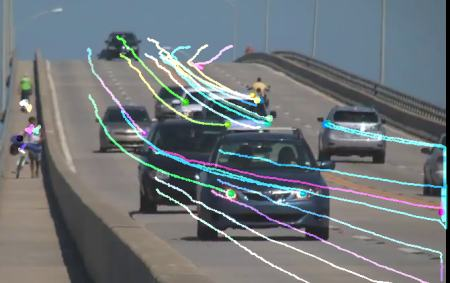
\includegraphics[width=0.5\linewidth]{figures/theoretical_foundations/opticalflow_lk.jpg}}
    \caption[Sparse optical flow]{An illustration of a sparse optical flow computed by the Lucas-Kanade algorithm~\cite{Lucas1981} across multiple frames. The drawn lines represent a trajectory of specifically selected features. Computation of the sparse optical flow also requires specific features to track. Those features can be determined by a plethora of algorithms, and one such a candidate is the handily named \emph{good features to track}~\cite{Shi1994} algorithm. \externalsrc{\cite{opticalflowimage}}}
    \label{fig:OpticalFlowLucasKanade}
\end{figure}

When estimating the optical flow, time starts to play a role. Besides, there are two assumptions upon which these algorithms operate:
\begin{enumerate}
    \item there is no change in pixel intensity between the two consecutive frames,
    \item motion is similar in neighboring pixels.
\end{enumerate}
Thus, let $\func{I}{x, y, t}$ be the coordinates of some pixel in the considered image. Assume this pixel moves by a distance $\Delta x$ and $\Delta y$ in $x$ and $y$ direction, respectively. Let $\Delta t$ stand for the time the movement took between the previous and current frame. Given the assumptions above, we have the relation
\begin{equation}
    \func{I}{x, y, t} = \func{I}{x + \Delta x, y + \Delta y, t + \Delta t}.
\end{equation}
Taking the Taylor expansion of the right-hand side produces the equation
\begin{equation}
    \frac{\partial I}{\partial x} \Delta x +
    \frac{\partial I}{\partial y} \Delta y +
    \frac{\partial I}{\partial t} \Delta t =
    0,
\end{equation}
where division by the $\Delta t$ term yields
\begin{equation}
    \frac{\partial I}{\partial x} \frac{\Delta x}{\Delta t} +
    \frac{\partial I}{\partial y} \frac{\Delta y}{\Delta t} +
    \frac{\partial I}{\partial t} = 0,
\end{equation}
and after substitution
\begin{equation}
    \label{eq:OpticalFlowEquation}
    \frac{\partial I}{\partial x} \nu_x +
    \frac{\partial I}{\partial y} \nu_y +
    \frac{\partial I}{\partial t} =
    0.
\end{equation}

Gradients of the image with respect to $x$, $y$ and $t$, represented by $\frac{\partial I}{\partial x}$, $\frac{\partial I}{\partial y}$ and $\frac{\partial I}{\partial t}$, can be easily obtained. However, there are two unknowns, namely $\nu_x$ and $\nu_y$ (main components of the velocity, or the optical flow of the image $\func{I}{x, y, t}$) the values of which cannot be solved because only one equation is available. To this end, various methods have been proposed, and equation~\ref{eq:OpticalFlowEquation} is appropriately called the \emph{optical flow equation}~\cite{fleet2006optical}.
